% 3D Surface and Parametric Plots
% Demonstrates: pgfplots 3D surfaces, contour plots, and parametric curves.
% Compile with: pdflatex main.tex
% Requires: pgfplots >= 1.16

\documentclass{article}
\usepackage{pgfplots}
\pgfplotsset{compat=1.18}
\usepgfplotslibrary{colormaps}

\title{3D Plots with PGFPlots}
\author{LaTeX Tutorial}
\date{\today}

\begin{document}
\maketitle

% =============================================================================
\section{Surface Plot}
% =============================================================================

A surface defined by $f(x,y) = \sin(\sqrt{x^2 + y^2})$:

\begin{center}
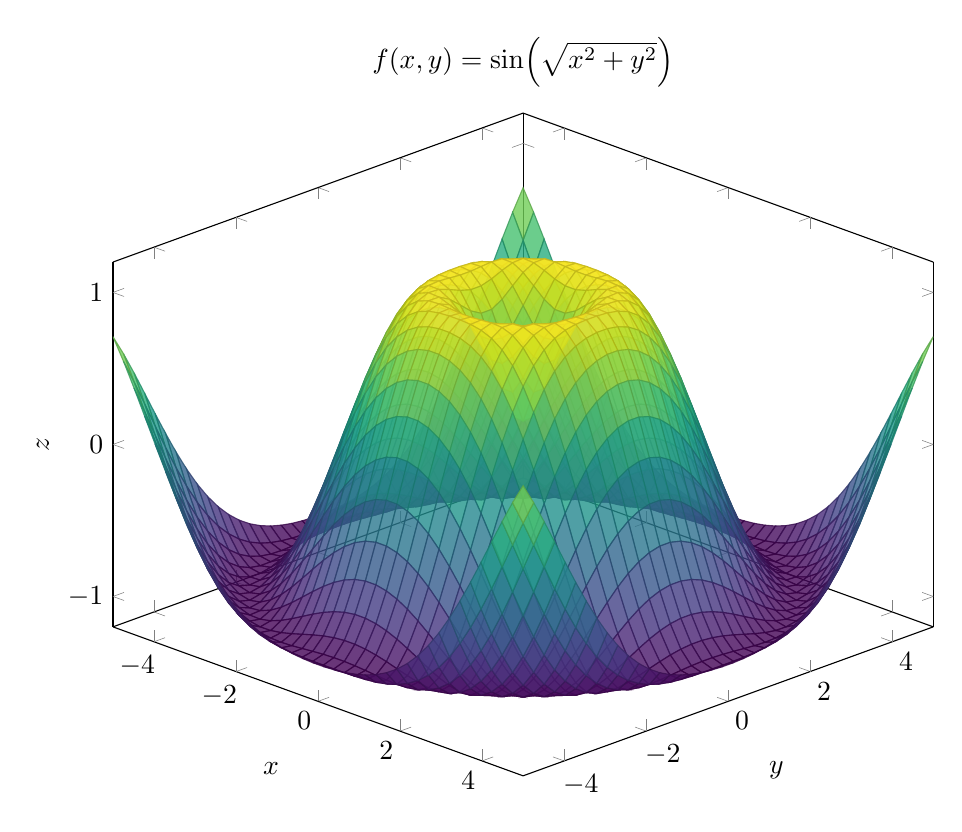
\begin{tikzpicture}
\begin{axis}[
    title={$f(x,y) = \sin\!\left(\sqrt{x^2+y^2}\right)$},
    xlabel={$x$}, ylabel={$y$}, zlabel={$z$},
    width=12cm, height=10cm,
    view={45}{30},
    colormap/viridis,
    mesh/rows=40,
]
    \addplot3[surf, domain=-5:5, domain y=-5:5, samples=40, opacity=0.8]
        {sin(deg(sqrt(x^2 + y^2)))};
\end{axis}
\end{tikzpicture}
\end{center}

% =============================================================================
\section{Saddle Surface}
% =============================================================================

The hyperbolic paraboloid $z = x^2 - y^2$:

\begin{center}
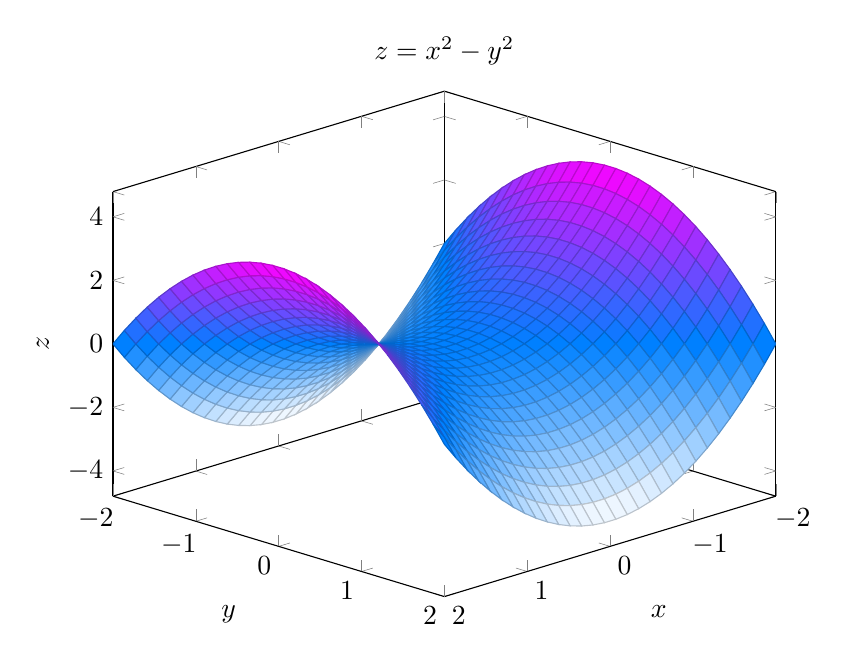
\begin{tikzpicture}
\begin{axis}[
    title={$z = x^2 - y^2$},
    xlabel={$x$}, ylabel={$y$}, zlabel={$z$},
    width=10cm, height=8cm,
    view={135}{25},
    colormap/cool,
]
    \addplot3[surf, domain=-2:2, domain y=-2:2, samples=30]
        {x^2 - y^2};
\end{axis}
\end{tikzpicture}
\end{center}

% =============================================================================
\section{Parametric 3D Curve}
% =============================================================================

A helix: $\bigl(\cos(t),\; \sin(t),\; t/4\bigr)$ for $t \in [0, 6\pi]$:

\begin{center}
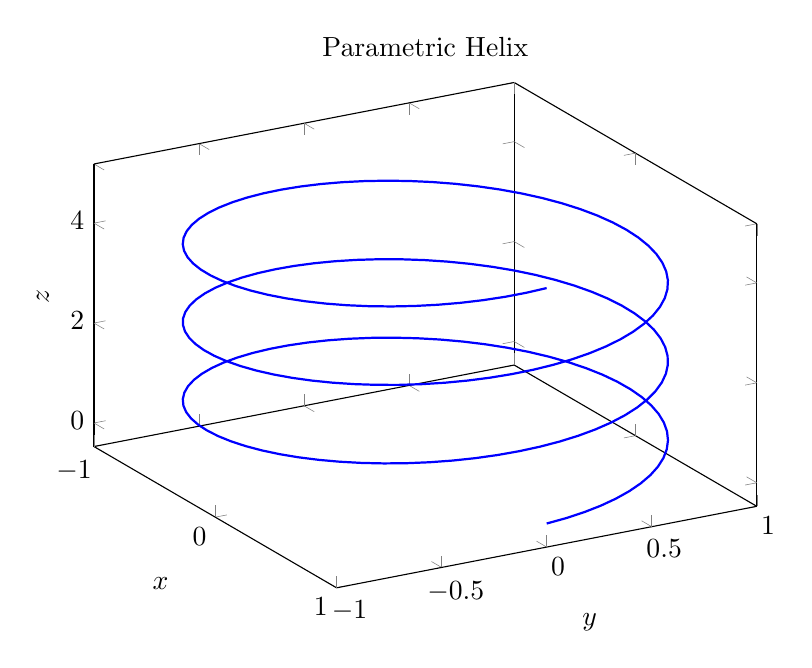
\begin{tikzpicture}
\begin{axis}[
    title={Parametric Helix},
    xlabel={$x$}, ylabel={$y$}, zlabel={$z$},
    width=10cm, height=8cm,
    view={60}{30},
]
    \addplot3[
        thick, blue, no marks,
        domain=0:6*pi, samples=200, samples y=0,
    ] ({cos(deg(x))}, {sin(deg(x))}, {x/4});
\end{axis}
\end{tikzpicture}
\end{center}

% =============================================================================
\section{Contour Plot}
% =============================================================================

Contour lines of $f(x,y) = x^2 + y^2$:

\begin{center}
\begin{tikzpicture}
\begin{axis}[
    title={Contour: $x^2 + y^2$},
    xlabel={$x$}, ylabel={$y$},
    width=10cm, height=8cm,
    view={0}{90},
    colormap/hot,
]
    \addplot3[contour gnuplot={
        levels={1, 2, 4, 8, 12, 16},
        draw color=black,
    }, domain=-4:4, domain y=-4:4, samples=40]
        {x^2 + y^2};
\end{axis}
\end{tikzpicture}
\end{center}

\end{document}
